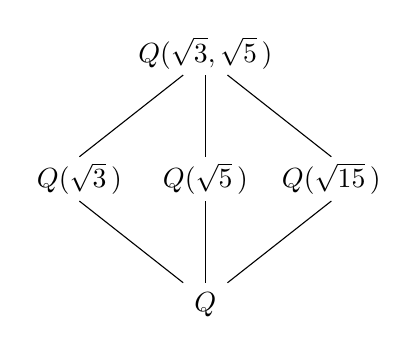
\begin{tikzpicture}[scale=0.8] 

\coordinate (Q-3-5) at (9,2);
\coordinate (Q-3) at (7,0);
\coordinate (Q-5) at (9,0);
\coordinate (Q-15) at (11,0);
\coordinate (Q) at (9,-2);

\node at (Q-3-5)  {${\mathbb Q}(\sqrt{3}, \sqrt{5}\, )$};
\node at (Q-3)  {${\mathbb Q}(\sqrt{3}\, )$};
\node at (Q-5)  {${\mathbb Q}(\sqrt{5}\, )$};
\node at (Q-15)  {${\mathbb Q}(\sqrt{15}\, )$};
\node at (Q)  {${\mathbb Q}$};

\draw  ([yshift=-10]Q-3-5) -- ([yshift=10]Q-5);
\draw  ([yshift=-10]Q-5) -- ([yshift=10]Q);
\draw  ([xshift=-10,yshift=-10]Q-3-5) -- ([yshift=10]Q-3);
\draw  ([xshift=10,yshift=-10]Q-3-5) -- ([yshift=10]Q-15);
\draw  ([yshift=-10]Q-3) -- ([xshift=-10,yshift=10]Q);
\draw  ([yshift=-10]Q-15) -- ([xshift=10,yshift=10]Q);

\end{tikzpicture}
